\feelchapter{Getting Started with Feel++}
            {Getting Started with Feel++}
            {Christophe Prud'homme, Baptiste Morin}
            {cha:getting-started}


\section{Creating applications}
\label{sec:creat-appl}


\marginpar{\lstinline!myapp.cpp!}

\subsection{Application and Options}
\label{sec:options}

As a \feel user, the first step in order to use \feel is to create an
application. Before writing anything, you have to include the \lstinline!Application! header and the header which handles the internal \feel options.
%\lstinline!feel/feelcore/application.hpp! and the header which the internal \feel options.
Note that \feel uses the \lstinline!boost::program_options!\footnote{\url{http://www.boost.org/doc/html/program_options.html}} (\verb|po|)
library from Boost to handle its command line options.

\lstinputlisting[linerange=marker1-endmarker1]{tutorial/myapp.cpp}

Next to ease the programming and reading, we use the \lstinline!using!
\cpp directive to bring the namespace Feel to the current namespace

\begin{lstlisting}
  using namespace Feel;
\end{lstlisting}

Then we define the command line options that the applications will
provide. Note that on the \lstinline!return! line, we incorporate the
options defined internally in \feel.

\lstinputlisting[linerange=marker2-endmarker2]{tutorial/myapp.cpp}

In the example, we provide the options \lstinline!dt! which takes an
argument, a \lstinline!double! and its default value is \lstinline!1!
if the options is not set by the command line. Then we describe the application by defining a class
\lstinline!AboutData! which will be typically used by the
\lstinline!help! command line options to describe the application


\lstinputlisting[linerange=marker3-endmarker3]{tutorial/myapp.cpp}


Now we turn to the class \lstinline!MyApp! itself: it derives from
\lstinline!Feel::Application!. This class provides two constructors : one with only description and one with additionnal parameters which enables to add options
\lstinline!argc! and \lstinline!argv!.
%and the \lstinline!AboutData! as well as possibly the description of the command line options \lstinline!Feel::po::option_description!.
This class \lstinline!MyApp! has to redefine the \lstinline!run()! method. It is defined as a pure virtual function in \lstinline!Application!.


\lstinputlisting[linerange=marker4-endmarker4]{tutorial/myapp.cpp}

The implementation of the constructors is usually simple, we pass the
arguments to the super class \lstinline!Application! that will analyze
them and subsequently provide them with a
\lstinline!Feel::po::variable_map! data structure which operates like
a \lstinline!map!. Have a look at the document \lstinline!boost::program_options!\footnote{\url{http://www.boost.org/doc/html/program_options.html}} for further details. Here our two constructors do nothing ( because $\{ \}$).

\lstinputlisting[linerange=marker5-endmarker5]{tutorial/myapp.cpp}

The \lstinline!run()! member function holds the application
commands/statements. Here we provide the smallest code unit: we print
the description of the application if the \lstinline!--help! command
line options is set.

\lstinputlisting[linerange=marker6-endmarker6]{tutorial/myapp.cpp}

Finally the \lstinline!main()! function can be implemented. We pass
the results of the \lstinline!makeAbout()! and
\lstinline!makeOptions()! to the constructor of \lstinline!MyApp! as
well as \lstinline!argc! and \lstinline!argv!. Then we call the
\lstinline!run()! member function to execute the application.

\lstinputlisting[linerange=marker7-endmarker7]{tutorial/myapp.cpp}

Now, you can check if your first \feel application is working. To compile \lstinline!myapp!, type in a command-line :
\begin{unixcom}
		cd feel.opt/doc/manual
		make feel_doc_myapp
\end{unixcom}

You are now able to execute it (obviously here \verb|./feel_doc_myapp| won't produce anything but you can try it to check the execution is ok)

\begin{lstlisting}[language=sh]
> ./feel_doc_myapp --help
myapp: my first Feel application
Allowed options:

MyApp options:
  --dt arg (=1)                              time step value

>./feel_doc_myapp --authors
myapp: my first Feel application
          Author Name       Task                          Email Address
-----------------------------------------------------------------------
Christophe Prud'homme   developer  christophe.prudhomme@ujf-grenoble.fr
\end{lstlisting}

\subsection{Application, Logging, Archiving, Configuring}
\label{sec:appl-logg-arch}

\feel provides some basic logging and archiving support: using the
\lstinline!changeRepository! member functions of the class
\lstinline!Application!, the logfile and results of the application
will be stored in a subdirectory of \lstinline!~/feel!. For
example the following code

\lstinputlisting[linerange=marker8-endmarker8]{tutorial/myapp.cpp}

will create the directory \lstinline!~/feel/doc/tutorial/! and will store the
logfile and any files created after calling
\lstinline!changeRepository!. Refer to the documentation of
\lstinline!Boost::format! of further details about the arguments to be
passed to \lstinline!changeRepository!. The logfile is named
\lstinline!~/feel/doc/tutorial/myapp-1.0!. The name of the logfile is built
using the application name, here \lstinline!myapp!, the number of
processes, here 1 and the id of the current process, here 0.

\paragraph{Configuring}

Each application can be configured via the command line but also using a
\verb|.cfg| file. If they exist they may have been installed on your system
along with \feel or you may create your own configuration files.  \feel provides
a way to look for them and parse them.

The \verb|.cfg| file is searched in the following order
\begin{enumerate}
\item look in the current directory
\item look in the directory \verb|$HOME/feel/config/|
\item look in the directory \verb|$INSTALL_PREFIX/share/feel/config/|,
  \emph{e.g.} in\\ Debian \verb|/usr/share/feel/config/|
\end{enumerate}
The name of the file can be constructed in two ways \verb|<appname>.cfg| and
\verb|feel_<appname>.cfg| where \verb|<appname>| is the string given in the
\verb|AboutData| data structure passed to the construction of the
\verb|Application| class.
Here are two examples of the logfiles in the case that there was not \verb|myapp.cfg| created.

\begin{lstlisting}[language=sh]
> ./feel_doc_myapp
> cat ~/feel/doc/tutorial/myapp/myapp-1.0
myapp-1.0 is opened for debug
the value of dt is 1
the value of myapp-solver-type is gmres
the value of myapp-pc-type is lu

> ./feel_doc_myapp --dt=0.2
> cat ~feel/doc/tutorial/myapp/myapp-1.0
myapp-1.0 is opened for debug
the value of dt is 0.2
the value of myapp-solver-type is gmres
the value of myapp-pc-type is lu
\end{lstlisting}

If you want to create a configured file, you have to create \verb|myapp.cfg| such as, for example :
\begin{lstlisting}[language=sh]
dt=1e-5
myapp-solver-type=cg
myapp-pc-type=ilu
\end{lstlisting}
This configured file will be parsed automatically before being executed. In that way you won't have to enter each time values you want to fix.


\subsubsection{MPI Application}

\marginpar{\lstinline!mympiapp.cpp!}

\feel relies on MPI for parallel computations and the class
\lstinline!Application!  initialises the MPI environment, for that, you should go to the appropriate repertory and call \lstinline!ccmake .!. Then turn on the \lstinline!FEELPP_ENABLE_MPI_MODE!
To launch a parallel computation for your application, you have to call the application \verb|mpirun| such as
\begin{lstlisting}[language=sh]
mpirun -np 2 mympiapp
\end{lstlisting}

\begin{lstlisting}[language=sh]
> cat ~/feel/mympiapp/mympiapp-2.0
mympiapp-2.0 is opened for debug
[Area 0] the value of dt is 1
[Area 0] we are on processor eta
[Area 0] this is process number 0 out of 2
> cat ~/feel/mympiapp/mympiapp-2.1
mympiapp-2.1 is opened for debug
[Area 0] the value of dt is 1
[Area 0] we are on processor eta
[Area 0] this is process number 1 out of 2

> mpirun -np 2 mympiapp --dt=0.01
> cat ~/feel/mympiapp/mympiapp-2.0
mympiapp-2.0 is opened for debug
[Area 0] the value of dt is 0.01
[Area 0] we are on processor eta
[Area 0] this is process number 0 out of 2
> cat ~/feel/mympiapp/mympiapp-2.1
mympiapp-2.1 is opened for debug
[Area 0] the value of dt is 0.01
[Area 0] we are on processor eta
[Area 0] this is process number 1 out of 2
\end{lstlisting}


\subsection{Initializing PETSc and Trilinos}

\index{PETSc}\index{Trilinos}\index{Libraries!PETSc}\index{Libraries!Trilinos}

PETSc is a suite of data structures and routines for the scalable (parallel)
solution of scientific applications modeled by partial differential
equations. It employs the MPI standard for parallelism.  

The Trilinos Project is an effort to develop algorithms and enabling
technologies within an object-oriented software framework for the solution of
large-scale, complex multi-physics engineering and scientific problems.

\feel supports the PETSc and Trilinos framework, the class
\lstinline!Application!\index{Class!Application} takes care of initialize the
associated environments. 


\section{Mesh Manipulation}
\marginpar{\lstinline!mymesh.cpp!}
\label{sec:mesh-manipulation}

\index{mesh}\index{Class!Mesh}

In this section, we present some of the mesh definition and
manipulation tools provided by \feel.

\subsection{Mesh definition}

We look at the definition of a mesh data structure. First, we define
the type of geometric entities that we shall use to form our mesh. \feel supports several geometric entities
\begin{itemize}
\item simplices: segment, triangle, tetrahedron
\item tensorized entities: segment, quadrangle, hexahedron
\end{itemize}

To create a mesh, use the following keywords \lstinline!Simplex<Dim,Order,RealDim>!  and \\
\lstinline!SimplexProduct <Dim,Order,RealDim>!. They have the same template
arguments:
\begin{itemize}
\item \lstinline!Dim!: the topological dimension of the entity (optional, default value = 1).
\item \lstinline!Order!: the order of the entity(usually 1, higher order in development).
\item \lstinline!RealDim!: the dimension of the real space (optional, default value = \lstinline!Dim!).
\end{itemize}


\lstinputlisting[linerange=marker1-endmarker1]{tutorial/mymesh.cpp}

Now, you are able to define the mesh type, \lstinline!Mesh<Entity>! by passing as
argument the type of entity it is formed with (at the moment hybrid
meshes are not supported).

\lstinputlisting[linerange=marker2-endmarker2]{tutorial/mymesh.cpp}

\lstinline!boost::shared_ptr! allows to manipulate a pointer on a mesh. It is
customary, and usually a very good practice, to define the
\lstinline!boost::shared_ptr<>!  counterpart which is used actually in practice.

%We can now instantiate a new mesh data structure.

%\lstinputlisting[linerange=marker3-endmarker3]{tutorial/mymesh.cpp}

\subsection{Mesh file format}
The next step is to read some mesh files. \feel supports essentially the Gmsh mesh file format. It provides also some classes to manipulate Gmsh \lstinline!.geo! files and generate \lstinline!.msh! files. To begin, we use some helper classes and functions to generate a \lstinline!.geo! file.

\begin{itemize}
\item \lstinline!domain! is a function which allows to generate a \verb|.geo| string description of simple domains such as simplex and hypercube.

\item \lstinline!createGMSHMesh! is a function which allows to generate a mesh file \verb|.msh| automatically from a description file ( \verb|.geo| for example) by using the \verb|_desc| parameter and store the generated mesh into the \verb|_mesh| parameter allocated when calling the function.

\item \lstinline!GmshSimplexDomain! is a class which will enable you to create simplex domains (e.g segment, triangle or tetrahedron). It allows to modify
  	\begin{itemize}
	 \item the characteristic size of the mesh (default $h=0.1$)
  	\item the domain vertices (default is $(-1,-1,-1), (1,-1,-1), (-1,1,-1), (-1,-1,1)$)
  	\end{itemize}

\item \lstinline!GmshHypercubeDomain! is a class which will enable you to create hypercube domains (e.g cube) in 1,2 or 3D. It allows to modify
  	\begin{itemize}
  	\item the characteristic size of the mesh (default $h=0.1$)
  	\item the domain (default is the cube $[0;1]\times[0;1]\times[0;1]$)
  	\end{itemize}
\end{itemize}

%The call to \lstinline!setCharacteristicLength! allows to change the mesh size to \lstinline!M_meshSize! which was given for example on the command line using the \lstinline!Application! framework, see section~\ref{sec:creat-appl}. The call to \lstinline!generate! creates the \lstinline!.geo! file and generate the associated mesh. Note that \lstinline!fname! holds the name of the \lstinline!.msh! file, e.g. \lstinline!mymesh.msh!. \feel adds automatically the \lstinline!.msh!  extension. Also note the last argument of \lstinline!GmshTensorizedDomain!, it allows to change the type of geometric entities used to generate the mesh. Here we use \lstinline!Simplex!, we could have also used \lstinline!SimplexProduct! (quadrangle or hexahedron)

%Next we import the mesh using the \lstinline!ImporterGmsh!\index{mesh!import}\index{Class!ImporterGmsh} class as follows:

%lstinputlisting[linerange=marker5-endmarker5]{tutorial/mymesh.cpp}
%At this stage we are ready to use the mesh instance: we can for example export the mesh to a postprocessing format. Two formats are supported at the moment
%\begin{itemize}
%\item \lstinline!Ensight! (case and sos) which is supported by the
%  software Ensight\footnote{\url{http://www.ensight.com}} and
%  Paraview\footnote{\url{http://www.paraview.org}}
%\item \lstinline!Gmsh! which is post-processing format of Gmsh
%\end{itemize}

%The export stage reads as follows:

%\lstinputlisting[linerange=marker6-endmarker6]{tutorial/mymesh.cpp}

%In this example, we create a $\polyP{0}$ function space and save the
%piecewise constant function that associates to each element the
%process id it belongs to. In sequential, they all belong to processor
%0.  In a parallel setting, the mesh is partitioned using Metis and
%each element is associated with a corresponding processor. The figure
%\ref{fig:1} displays a partitioned mesh in two regions and the
%associated $\polyP{0}$ function.

%\begin{figure}[htbp]
% \centering
% 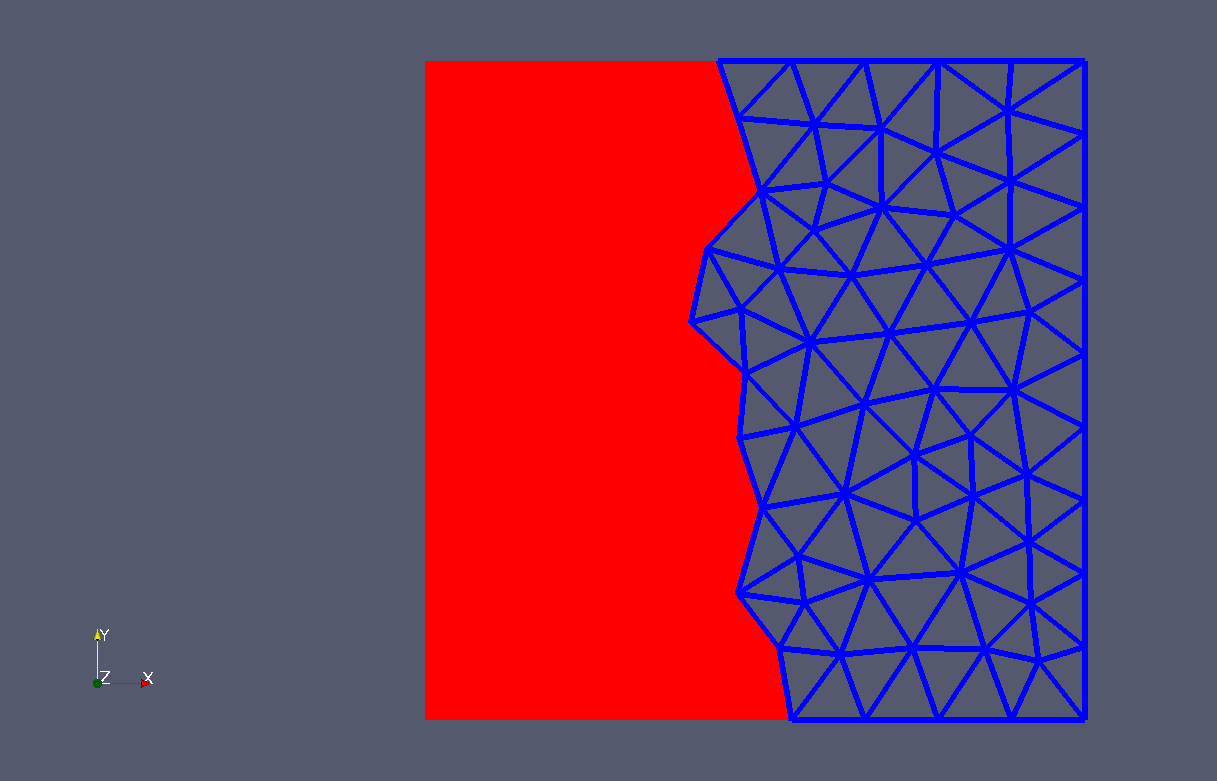
\includegraphics[width=.7\linewidth]{mymeshpartition}
%\label{fig:1}
%\caption{Screenshot of Paraview (3.2.1) of a 2D mesh partitioned and distributed on two processors}
%\end{figure}
\subsection{Examples}
\label{mesh:examples}
Here is an example of how to get a simplex or hypercube geometry :

\lstinputlisting[linerange=marker4-endmarker4]{tutorial/mymesh.cpp}
The parameter \lstinline!_h! in the function \lstinline!domain! allows to change the mesh characteristic size to \lstinline!M_meshsize! which is given for example on the command-line using the Application framework, please refer to ~\ref{sec:creat-appl} for more details. You can see the meshes, by executing with the followings ordering :

\begin{unixcom}
		./feel_doc_mymesh --shape=simplex
		./feel_doc_mymesh --shape=hypercube
\end{unixcom}
we generate some of the following graphics (which are located in \verb|~/feel/doc/tutorial/mymesh/| \newline \verb|hypercube-x/h_y.z| or \verb|~/feel/doc/tutorial/mymesh/simplex-x/h_y.z|)


To visualize the meshes, go to \lstinline!~/feel/doc/tutorial/mymesh/hypercube!
(or \lstinline!simplex!) and find out the \verb|.msh| files. Last step is to
launch gmsh with
\begin{unixcom}
  gmsh yourfile.msh
\end{unixcom}


\begin{figure}[!h]
  \centering
  \subfigure[Line in 1D]{
\includegraphics[width=4.5cm]{pngs/mymesh/hypercube_1.png}}
  \subfigure[Cube in 2D]{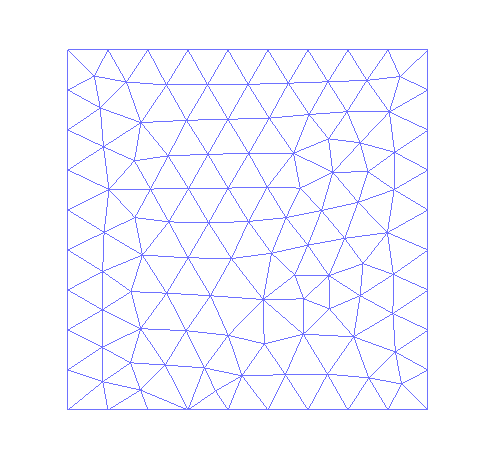
\includegraphics[width=4.5cm]{pngs/mymesh/hypercube_2.png}}
  \newline
  \centering
  \subfigure[Tetrahedron]{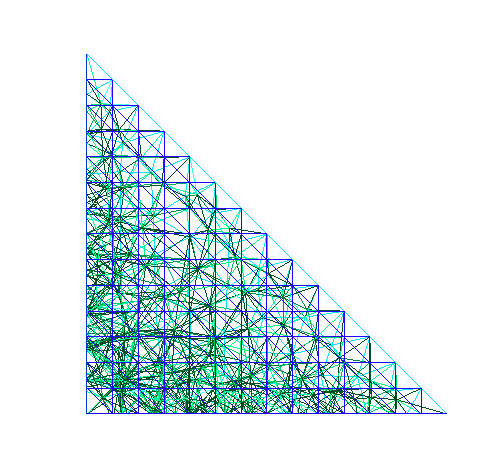
\includegraphics[width=4.5cm]{pngs/mymesh/simplex_3.png}}
  \subfigure[Unit cube in 3D]{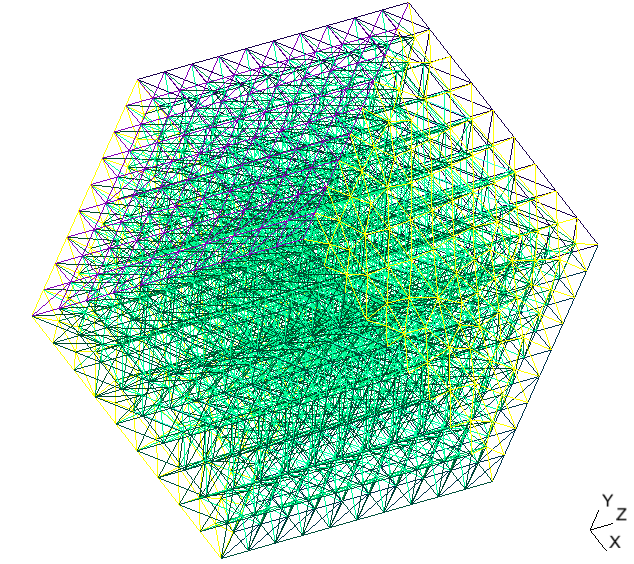
\includegraphics[width=4.5cm]{pngs/mymesh/hypercube_3.png}}
  \caption{Sequential computation}
\end{figure}
\label{fig:2}

Some examples of meshes generated in sequential and parallel computaion are shown in the following figures.


%%%%%%%%%%%%%%%%%%%%%%%%%%%%%%%%%%%%%%%%%%%%%%%%%%%%%%%%%%%%%%%%%%%%%%%%%%%%%%%%%%%%%%%%
 \begin{figure}[!h]
  \centering
  \subfigure[Square]{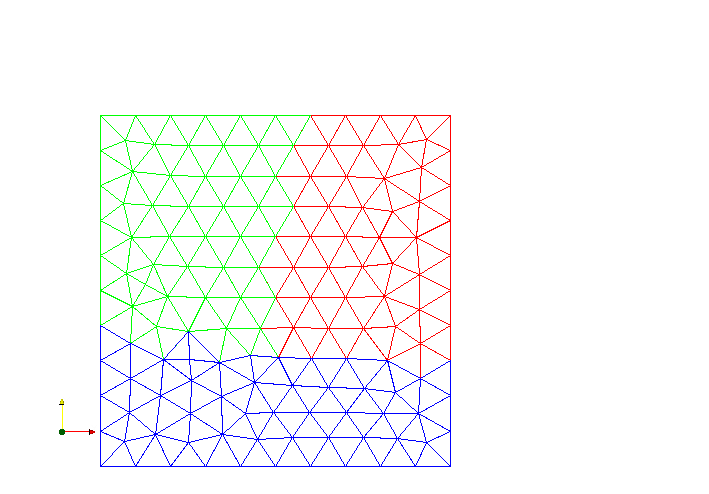
\includegraphics[width=4.75cm]{pngs/mymesh/mesh3.png}}
  \subfigure[Triangle]{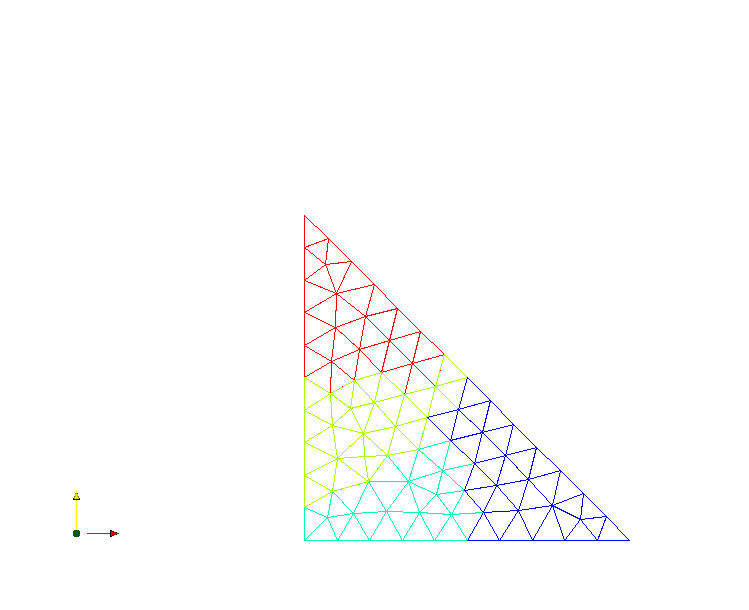
\includegraphics[width=4.75cm]{pngs/mymesh/mesh_triangle.png}}
  \subfigure[Cube in 3D]{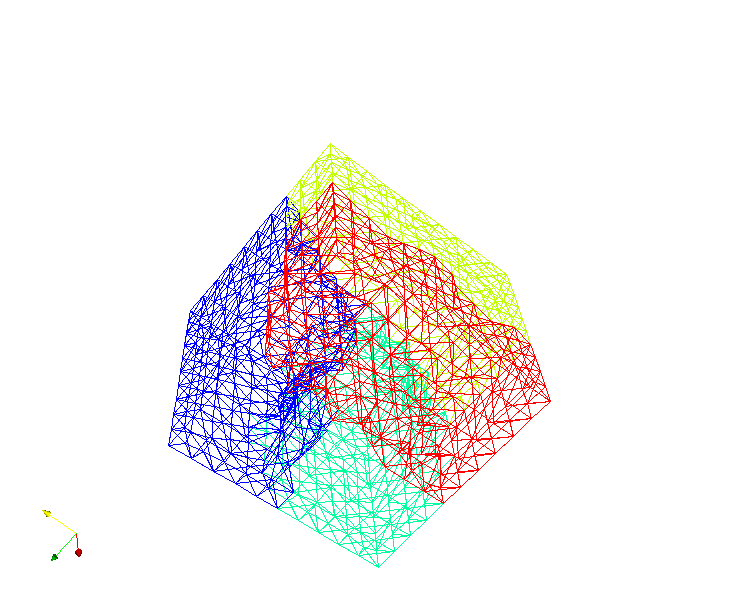
\includegraphics[width=4.75cm]{pngs/mymesh/mesh_cube.png}}
  \caption{Parallel computation for generating meshes}

\end{figure}
  \label{fig:2}

%%%%%%%%%%%%%%%%%%%%%%%%%%%%%%%%%%%%%%%%%%%%%%%%%%%%%%%%%%%%%%%%%%%%%%%%%%%%%%%%%%%%%%%%


\subsection{Exporting meshes for post-processing}

We can export the mesh to two postprocessing formats supported at the moment :
\begin{itemize}
\item \textbf{Ensight} (sos and case)  which is supported by the software Ensight and Paraview;
\item \textbf{Gmsh} which is post-processing format of Gmsh.
\end{itemize}

We define the exporter data structure type as follows :
\lstinputlisting[linerange=marker61-endmarker61]{tutorial/mymesh.cpp}

By default, the  export format is ensight. We can use the code \lstinline!Exporter::setMesh()! and \lstinline!Exporter::save()! to save the mesh to the format given to the command line --exporter= <format>

\lstinputlisting[linerange=marker62-endmarker62]{tutorial/mymesh.cpp}

To take into account the exporting format, you have to type thoses syntaxes
\begin{unixcom}
		./feel_doc_mymesh  --exporter= gmsh
		./feel_doc_mymesh  --exporter= paraview
\end{unixcom}


\subsection{Iterating over the entities of a mesh}

\feel mesh data structures provides powerful iterators that allows to
walk though the mesh in various ways: iterate over element, faces ,
points, marked\footnote{associated to an integer flag denoting a
  region, material, processor} elements, marked faces, ...

\subsection{Load meshes}
\marginpar{\lstinline!loadmesh.cpp!}

\feel supports gmsh meshes but not only, you can also wortk with medit (\lstinline!.mesh!) or STL (\lstinline!.stl!) files format. The full explaination is avaible in the HOW TO section you can find at \ref{howto:spec-meshes}. This is implemented in \lstinline!loadmesh.cpp! which is a simple application which loads a mesh and calculate its surface and volume.

\section{Computing integrals}
\label{sec:computing-integrals}
\marginpar{\lstinline!myintegrals.cpp!}

\subsection{Problem statement}

If you have followed this tutorial in the order, you are now able to create a simple application and generate meshes. We are now interested in computing integrals on the meshes we have generated. Let's consider this mesh (no matter which one) on a domain $\Omega$ and parts of the domain, i.e. subregions and (parts of) boundary. In this tutorial the domain can be either

\[ \Omega=[0,1]^d\ \subset\ \mathbb{R}^d \]

or

\[ \Omega=\{ \mathbf{x} \in \mathbb{R}^d | x_i \geq 0, \sum_{i=1}^{d} x_i \leq 1 \} \]

where $ d=1,2$ or $3$ and $\mathbf{x}=(x_1,...,x_d)$.

These domains are plotted in the section ~\ref{sec:mesh-manipulation} (If it's
not yet done, compile all examples which are used in this tutorial, go to
\lstinline!~/FEEL/feel.opt/doc/manual/! and type \verb|make| and execute the
application \verb|feel_doc_mymesh|). The execution will result in several meshes
as it is explained in ~\ref{mesh:examples}.

Here are the integrals we want to compute :
\begin{itemize}
\item $\displaystyle{ \int_\Omega 1 }$ : the measure of the domain
\item $\displaystyle{ \int_{\partial\Omega} 1 }$: the measure of the surface of the domain (Dim>1)
\item $ \displaystyle{\int_{\Omega} x^2+y^2+z^2 }$ : the integral over $\displaystyle{\Omega}$ of $ \displaystyle{(x,y,z) \mapsto x^2+y^2+z^2}$ with the convention that $y=z=0$ in 1D and $ z=0 $ in 2D.
\item $\displaystyle{ \int_{\Omega} sin(x^2+y^2+z^2)} $ : the integral over $\Omega$ of $\displaystyle{ (x,y,z) \mapsto sin(x^2+y^2+z^2)}$ with the same convention as above.
\end{itemize}

\subsection{Implementation}

To compute an integral, we use the following function
\begin{lstlisting}
integrate( <domain>,<expression under the integral> ).evaluate(<location>)
\end{lstlisting}

\subsubsection{Domain}

You have to indicate the domain on which we want to integrate. It consists in a pair of iterators over the elements owned by the current processor (the mesh is shared between the processors).
\begin{itemize}
\item To compute the integral over the region of $\Omega$ current processor, use
\begin{lstlisting}
elements(mesh)
\end{lstlisting}
\item To compute the integral on the boundary faces of the domain $\Omega$, use
\begin{lstlisting}
boundaryfaces(mesh)
\end{lstlisting}
\end{itemize}

\subsubsection{Expression under the integrals}

The language provided by \feel (called the Finite Element Embedded Language) brings the keyword $Px()$, $Py()$ and $Pz()$ to denote the $x$, $y$ and $z$ coordinates. \\
The expression $x^2 + y^2 + z^2$ under the third integral should be written such as :
\begin{lstlisting}
Px()*Px() + Py()*Py() + Pz()*Pz()
\end{lstlisting}
\vspace{0.2cm}
The constants are indicated by the function constant() (for example, we have to indicate \lstinline!constant(1.0)! for the first integral). \\

\subsubsection{Examples}

\paragraph{First integral : domain area \\}
To compute the first integral (the domain area) and to have the local contributions only, we have to pass 'false' to \lstinline!evaluate! as follows :
\lstinputlisting[linerange=marker1-endmarker1]{tutorial/myintegrals.cpp}


This compute the integral only on the region of the domain owned by the current processor \lstinline!(local_domain_area)!. \\

To obtain the total area,\lstinline!integrate(...).evaluate()! computes the global integral in parallel which induces communications (all\_reduce) to compute the sum of the local contributions \\
\lstinputlisting[linerange=marker2-endmarker2]{tutorial/myintegrals.cpp}

\vspace{0.2cm}
Finally, we print to the log file the result of the local and global integral calculation.
\lstinputlisting[linerange=marker3-endmarker3]{tutorial/myintegrals.cpp}

\paragraph{Second integral : domain perimeter \\}

The difference with the domain area computation resides in the elements with are iterating on: here we are iterating on the boundary faces of the domain to compute the integral using \lstinline!boundaryfaces(mesh)! to provide the pairs of iterators. But the stages are the same as previously \\

\lstinputlisting[linerange=marker4-endmarker4]{tutorial/myintegrals.cpp}

We can apply the same method to compute the third, and the last integral. \\

\subsection{Quadrature}

Feel computes automatically the quadrature associated to the expression under the integral. If the expression is polynomial then the quadrature is exact. If the expression is not polynomial, then each non-polynomial term in the expression is considered as a polynomial of degree 2 by default.

Here is how the 4-th integral can be computed letting Feel decide about the quadrature \\
\lstinputlisting[linerange=marker6-endmarker6]{tutorial/myintegrals.cpp}

An alternative is to set yourself the quadrature by passing a new argument to the integrate function: \_Q<Order>() where Order is the maximum polynomial order that the quadrature should integrate exactely.
\lstinputlisting[linerange=marker7-endmarker7]{tutorial/myintegrals.cpp}

\subsection{Complete example : application, mesh and integrals}

Here, we'll see how to build an application which create a mesh, and compute some integrals on it.

\subsubsection{Application building}
As we can see in the creating applications section (~\ref{sec:creat-appl}), we can add a description and some options to our new application.
Here, we have created two functions \lstinline!makeAbout()! and \lstinline!makeOptions()! which create respectively the descritpion and the list of options.
\lstinline!makeOptions()! creates a list of options (myintegralsoptions), and adds two options :
\begin{itemize}
\item \lstinline!hsize! which corresponds to the mesh size (default = $0.2$)
\item \lstinline!shape! which corresponds to the shape of the domain (default = $hypercube$)
\end{itemize}

\lstinputlisting[linerange=marker8-endmarker8]{tutorial/myintegrals.cpp}

makeAbout() gives the description of the application :\\

\lstinputlisting[linerange=marker9-endmarker9]{tutorial/myintegrals.cpp}

To get further information about the application, see creating applications section ~\ref{sec:creat-appl}.

\subsubsection{Class definition}

Once the description and options have been defined, we create the class Myintegrals, with the constructor \\
\begin{lstlisting}
MyIntegrals( po::variables_map const& vm, AboutData const& about )
\end{lstlisting}
which takes \lstinline!vm! (a map which associates the available options with their default value), and \lstinline!about! (containing our application's description). \\

The \lstinline!run()! member function is redifined twice in this class :
\lstinputlisting[linerange=marker10-endmarker10]{tutorial/myintegrals.cpp}
These two versions are linked, because the first uses the second. Indeed, \lstinline!run()! stores the parameters we have chosen with the options \lstinline!(mesh size, shape, $\dots$)!, and uses them in the second version (X corresponds to these parameters : \lstinline!X[0]=mesh_size! and \lstinline!X[1]=mesh_shape!). \\

\subsubsection{The run() member function}
In this function, we create a subdirectory of feel in which there will be the results of our application, and logfiles containing :
\begin{itemize}
\item the application's name
\item the mesh size
\item the mesh shape
\end{itemize}

\begin{lstlisting}
if ( !this->vm().count( "nochdir" ) )
Environment::changeRepository( boost::format( "doc/tutorial/%1%/%2%/h_%3%/")
                                  this->about().appName()
                                  shape
                                  meshSize );

\end{lstlisting}

It is also in run() that we create the mesh before to compute the integrals :
\lstinputlisting[linerange=marker11-endmarker11]{tutorial/myintegrals.cpp}
Now that we have a computational mesh, we can compute the integrals as we have seen before :

\begin{lstlisting}
    double local_domain_area = integrate( elements(mesh),
                                        constant(1.0)).evaluate()(0,0);

    double global_domain_area=local_domain_area;
    if ( this->comm().size()  > 1 )
        mpi::all_reduce( this->comm(),
                         local_domain_area,
                         global_domain_area,
                         std::plus<double>() );

    Log() << "int_Omega 1 = " << global_domain_area
          << "[ " << local_domain_area << " ]\n";
\end{lstlisting}

\subsection{Results}

After compiling \lstinline!feel_doc_myintegrals! with the defaults options
\begin{lstlisting}
  --hsize arg (=0.20000000000000001)    mesh size
  --shape arg (=hypercube)              shape of the domain
\end{lstlisting}

we obtain the values of each integrals, in each dimension ($1,2$ and $3$) : \\
\begin{lstlisting}
------------------------------------------------------------
Execute MyIntegrals<1>
int_Omega 1 = 1[ 1 ]
int_Omega (x^2+y^2+z^2) = 0.333333[ 0.333333 ]
int_Omega (sin(x^2+y^2+z^2)) [with order 4 max exact integration]= 0.310268[ 0.310268 ]
int_Omega (sin(x^2+y^2+z^2)) [with order 2 max exact integration] = 0.310281[ 0.310281 ]
------------------------------------------------------------
Execute MyIntegrals<2>
int_Omega 1 = 1[ 1 ]
int_BoundaryOmega (1)= 4[ 4 ]
int_Omega (x^2+y^2+z^2) = 0.666667[ 0.666667 ]
int_Omega (sin(x^2+y^2+z^2)) [with order 4 max exact integration]= 0.56129[ 0.56129 ]
int_Omega (sin(x^2+y^2+z^2)) [with order 2 max exact integration] = 0.561299[ 0.561299 ]
------------------------------------------------------------
Execute MyIntegrals<3>
int_Omega 1 = 1[ 1 ]
int_BoundaryOmega (1)= 6[ 6 ]
int_Omega (x^2+y^2+z^2) = 1[ 1 ]
int_Omega (sin(x^2+y^2+z^2)) [with order 4 max exact integration]= 0.731683[ 0.731683 ]
int_Omega (sin(x^2+y^2+z^2)) [with order 2 max exact integration] = 0.731693[ 0.731693 ]
\end{lstlisting}



%%%%%%%%%%%%%%%%%%%%%%%%%%%%%%%%%%%%%%%%%%%%%%%%%%%%%%%%%%%%%%%%%%%%%%%%%%%%%%%%%%%%%%%%%%%%
This application can be executed in parallel as well. The results in dimension 2 of each integral are as follow : 
\begin{lstlisting}
------------------------------------------------------------
Execute MyIntegrals<2>
int_Omega 1 = 1[ 0.353404 ]
int_BoundaryOmega (1)= 4[ 1.5 ]
int_Omega (x^2+y^2+z^2) = 0.666667[ 0.0801182 ]
int_Omega (sin(x^2+y^2+z^2)) [with order 4 max exact integration]= 0.56129
int_Omega[0] (sin(x^2+y^2+z^2)) [with order 4 max exact integration]= 0.0787206
int_Omega (sin(x^2+y^2+z^2)) [with order 2 max exact integration] = 0.561298[ 0.0787224 ]

int_Omega 1 = 1[ 0.336194 ]
int_BoundaryOmega (1)= 4[ 0.75 ]
int_Omega (x^2+y^2+z^2) = 0.666667[ 0.247545 ]
int_Omega (sin(x^2+y^2+z^2)) [with order 4 max exact integration]= 0.56129
int_Omega[1] (sin(x^2+y^2+z^2)) [with order 4 max exact integration]= 0.221861
int_Omega (sin(x^2+y^2+z^2)) [with order 2 max exact integration] = 0.561298[ 0.221865 ]

int_Omega 1 = 1[ 0.310402 ]
int_BoundaryOmega (1)= 4[ 1.75 ]
int_Omega (x^2+y^2+z^2) = 0.666667[ 0.339003 ]
int_Omega (sin(x^2+y^2+z^2)) [with order 4 max exact integration]= 0.56129
int_Omega[2] (sin(x^2+y^2+z^2)) [with order 4 max exact integration]= 0.260709
int_Omega (sin(x^2+y^2+z^2)) [with order 2 max exact integration] = 0.561298[ 0.26071 ]
\end{lstlisting}

%%%%%%%%%%%%%%%%%%%%%%%%%%%%%%%%%%%%%%%%%%%%%%%%%%%%%%%%%%%%%%%%%%%%%%%%%%%%%%%%%%%%%%%%%%%


\section{Function Spaces}

\label{sec:func-spaces}
\marginpar{\lstinline!myfunctionspace.cpp!}

\subsection{Functions spaces definition}

In order to resolve partial derivative equations, we have to define the function space on which we work.
We can define a new type \lstinline!space_type! which corresponds to our new functions space
\begin{lstlisting}
 typedef FunctionSpace<mesh_type, basis_type> space_type;
\end{lstlisting}
To define this function space, we have to define :
\begin{itemize}
 \item \lstinline!mesh_type! the mesh on which we work (see~\ref{sec:mesh-manipulation})
 \item \lstinline!basis_type! the base of the function space (see~\ref{sec:base-funct})
\end{itemize}

\underline{Remark} : We can use the librairie Boost.smartptr of Boost, which has a reference counter (in the shared\_ptr class). It permits
to manage the memory (if we have built an object and that there are no more any pointers on it, it is automatically destructed).

\subsubsection{Base of the function space}
\label{sec:base-funct}
To define the base of functions we want to use, we have to indicate :
\begin{itemize}
 \item The type of the polynomials ($\mathbb{P}$) we want to use
 \begin{itemize}
   \item \lstinline!Lagrange! (more used than the others because more customizable)
   \item \lstinline!Legendre! (only for hypercube)
   \item \lstinline!Dubiner! (only for simplex)
   \item \lstinline!Crouzeix-Raviart!
   \item \lstinline!Raviart-Thomas!
 \end{itemize}

 \item The order of these polynomials (an integer in $\mathbb{N}^*$)
 \item The dimension of Im(P) (\lstinline!Scalar! if Im($\mathbb{P})=\mathbb{R}$, \lstinline!Vectorial! if the dimension is up to $1$)
 \item The continuity of polynomials at the interface ( \lstinline!Continuous! or \lstinline!Discontinuous!)
\end{itemize}
After we have chosen this parameters, we can create the new function base (new type \lstinline!basis_type!) :
\begin{lstlisting}
 typedef bases<Lagrange<0,Scalar,Discontinuous> > basis_type;
\end{lstlisting}

Here, we build a base with Lagrange polynomials, with order 0. The result of these polynomials is a scalar, and we authorized them
to be discontinue at the interface between two elements. In our example, \lstinline!p0_space_type! is the function space that holds piecwise constant $\mathbb{P}_0$ functions :  \\
\lstinputlisting[linerange=marker1-endmarker1]{tutorial/myfunctionspace.cpp}

\subsubsection{Instantiation of the function space}

We want now to instanciate the function space $X_h$ of type \lstinline!space_type! (that we created previously). \\

First, we build the mesh on which we want to work (of type \lstinline!mesh_ptrtype!)
\lstinputlisting[linerange=marker31-endmarker31]{tutorial/myfunctionspace.cpp}

Then we instantiate $X_h$ using \lstinline!space_type::New()! static member function and obtain a \lstinline!space_ptrtype!.
\lstinputlisting[linerange=marker32-endmarker32]{tutorial/myfunctionspace.cpp}
We are now able to instanciate elements on $X_h$. There are two ways to proceed, using auto keyword allowing to infer automatically the type of $ X_h$ elements or knowing the actual type of the elements
\lstinputlisting[linerange=marker33-endmarker33]{tutorial/myfunctionspace.cpp}

\subsection{Using function space and functions}
\subsubsection{Projection}

First, we define some mathematical expression/functions
\begin{eqnarray*}
g(x,y,z) &=& \sin(\pi x/2)\ \cos(\pi y/2)\ \cos(\pi*z/2) \\
f(x,y,z) &=& (1-x^2)\ (1-y^2)\ (1-z^2)\ (x^2+y^2+z^2)^{\alpha/2.0},\quad \alpha=3
\end{eqnarray*}
In our example, these functions correspond to
\lstinputlisting[linerange=marker4-endmarker4]{tutorial/myfunctionspace.cpp}
(they are implemented using the new \lstinline!auto! C++ keyword to infer the type of expression automatically). \\ \\
Then we build the interpolant (Lagrange interpolant in this case since we chose Lagrange basis function), by calling the \lstinline!vf::project()! function which can be applied on all or parts of the mesh thanks to the mesh iterators such as \lstinline!elements(mesh)! or \lstinline!markedelements(mesh,marker)!.
The return object is the interpolant of the function in the space $ X_h $ given as an argument to \lstinline!vf::project()!.
\lstinputlisting[linerange=marker5-endmarker5]{tutorial/myfunctionspace.cpp}
Here, $u$ is the projection of $g$ on the nodes of the mesh. Note that $u$ and $g$ have not the same type. To evaluate the error of $(u-g)$ on the nodes, we have to evaluate the function $u$, with the function $v$.

\subsubsection{Norm}

To calculate norms, we use integrals. For example, the $L_2$ norm is defined by :
$$\displaystyle{\| g\|_{L_2} = \sqrt{\int_\varOmega (g)^2}}$$
To compute this, we use the integrate function (See ~\ref{sec:computing-integrals}) with \lstinline!elements(mesh)! which allows to integrate on the entire domain.
Let's see an example of norms computation with log file printing :
\lstinputlisting[linerange=marker6-endmarker6]{tutorial/myfunctionspace.cpp}


\subsection{Results}

\subsubsection{Execution without option}

We have made a test code (it is still \verb|myfunctionspace.cpp| which create a new application myfunctionspace with some options (added with a \lstinline!makeOptions()! function),
and a description (with a \lstinline!makeAbout()! function). (See~\ref{sec:creat-appl}). \\

This code applies the examples we have seen previously, and when we execute it without option, we obtain :

\begin{lstlisting}
Execute MyFunctionSpace<2>
||u-g||_0=0.00463274
||v-f||_0=0.000483591
---------------------------------------------------
Execute MyFunctionSpace<3>
||u-g||_0=0.00968019
||v-f||_0=0.000474499
\end{lstlisting}
As we have seen before, $u$ is the projection of $g$ in the function space. So on the mesh nodes, the error's norm has to be
zero (the results we obtain here don't seems to be coherent).


%\subsection{Using functions spaces and functions}

%\begin{itemize}
%\item interpolating
%\item nodal projection
%\item saving
%\end{itemize}


\section{Linear Algebra}
\label{sec:linear-algebra}

\feel supports three different linear algebra environments that we
shall call \emph{backends}.
\begin{itemize}
\item Gmm%\footnote{}
\item Petsc\footnote{Petsc is a suite of data structures and routines for the scalable solution of scientific applications modeled by PDE available at \url{http://www.mcs.anl.gov/petsc/petsc-as/}}
\item Trilinos\footnote{The Trilinos Project is an effort to develop algorithms and enabling technologies within an object-oriented software framework for scientific problems. \url{http://trilinos.sandia.gov/}}
\end{itemize}


\subsection{Choosing a linear algebra backend}
\label{sec:choos-line-algebra}

\index{Class!Backend}\index{boost!shared\_ptr}
To select a backend in order to solve a linear system, we instantiate
the \lstinline!Backend! class associated :
\begin{lstlisting}
#include <feel/feelalg/backend.hpp>
boost::shared_ptr<Backend<double> > backend =
     Backend<double>::build( BACKEND_PETSC );
\end{lstlisting}
The backend provides an interface to solve
\begin{equation}
  \label{eq:8}
  A x = b
\end{equation}
where $A$ is a $n \times n $ sparse matrix and $x,b$ vectors of size $n$. The backend defines the \cpp types for  each of these, e.g :
\begin{lstlisting}
Backend<double>::sparse_matrix_type A;
Backend<double>::vector_type x,b;
\end{lstlisting}
In practice, we use the \lstinline!boost::shared_ptr<>! shared pointer
to ensure that we won't get memory leaks. The backends provide a
corresponding \lstinline!typedef!

\begin{lstlisting}
Backend<double>::sparse_matrix_ptrtype A( backend->newMatrix( Xh, Yh ) );
Backend<double>::vector_ptrtype x( backend->newVector( Yh ) );
Backend<double>::vector_ptrtype b( backend->newVector( Xh ) );
\end{lstlisting}
where $X_h$ and $Y_h$ are function spaces providing the number of
degrees of freedom that will define the size of the matrix and vectors
thanks to the helpers functions \lstinline!Backend::newMatrix()! and
\lstinline!Backend::newVector!. In a parallel setting, the
local/global processor mapping would be passed down by the function
spaces.

%\subsection{Defining and using matrices and vectors}
%\label{sec:defin-using-matr}

\subsection{Solving}
\label{sec:solving}

To solve the linear problem $Ax=b$, the backend provides a function \lstinline!solve! with three required parameters
\begin{lstlisting}
 solve(_matrix=A, _solution=x, _rhs=b)
\end{lstlisting}
where :
\begin{itemize}
\item the matrix $A$ has a \lstinline!sparse_matrix_ptrtype! type
\item the solution $x$ has a type \lstinline!vector_type! or \lstinline!vector_ptrtype!
\item the second member vector $b$ has a type \lstinline!vector_ptrtype!
\end{itemize}
You can also add optional parameters like :
\begin{itemize}

\item a preconditioner : instead of solving $Ax=b$, we solve $P^{-1}Ax= P^{-1}b$. This method can be applied in iterative methods and permits to decrease the number of iterations in the resolution system

\item a maximum number of iterations : this option is used with an iterative solving method

\item a residual tolerance : the fraction $\displaystyle{\frac{\mid\mid r^{(k)} \mid\mid }{\mid\mid r^{(0)} \mid\mid}}$ is inferior to the residual tolerance with
$r^{(k)}=b-Ax^{(k)}$ and $x^{(k)}$ the solution at the $k^{th}$ iteration

\item a absolute tolerance : $\mid\mid r^{(k)} \mid\mid $ is inferior to the absolute tolerance

\item a different tolerance : sometimes, the residue doesn’t decrease continuously during the iterations. The difference between two plots doesn’t have to exceed the parameter choosen for the difference tolerance.

\item a boolean to use transpose matrix : instead of solving $Ax=b$, we solve $A^{t}x=b$. If $A$ is defined and positive, $A^{t}=A$.

\end{itemize}

To have a view of the values of the optional parameters, see the following code :

\begin{lstlisting}
BOOST_PARAMETER_MEMBER_FUNCTION(
	(solve_return_type),
         solve,
         tag,
         (required
	(matrix,(sparse_matrix_ptrtype))
	(in_out(solution),*(mpl::or_<boost::is_convertible<mpl::_,vector_type&>,
                                         boost::is_convertible<mpl::_,vector_ptrtype> >))
	(rhs,(vector_ptrtype)))
	(optional
	  (prec,(sparse_matrix_ptrtype), matrix )
	  (maxit,(size_type), 1000 )
	  (rtolerance,(double), 1e-13)
	  (atolerance,(double), 1e-50)
	  (dtolerance,(double), 1e5)
	  (reuse_prec,(bool), false )
	  (transpose,(bool), false )
	  )
	)
    {
\end{lstlisting}

\noindent The library \lstinline!Boost::Parameters! allows you to enter parameters in the order you want. It supports deduced parameters,  that is to say parameters whose identity can be deduced from their types.

\section{Variational Formulation}
\label{sec:vari-form}
\index{formulation!variational}

\subsection{Principle}
\label{sec:vari-form-princip}
A variational formulation of a problem is also called weak formulation. The key
item is to bring a new function (called test function) and to integrate by
parts. In that way we decrease the regularity constraint on our functions.
%The finite elements method, on which is based $Feel++$ library, is used to numerically solve partial differential equation. The resolution of such equations makes the representation of complex system's dynamic behavior possible.

Let's consider the equation to solve with boundary conditions where $u  \in \varOmega$ is the unknown
\begin{equation}
\begin{array}{l l l}
	-\Delta u = f  \\
	u = u_D \quad on \quad \Gamma_D \\
	\nabla u.n = g \quad on \quad \Gamma_N
\end{array}
\end{equation}
$\Gamma = \Gamma_D \cup \Gamma_N$ is the border of $\varOmega$. By integrating by parts with a function $v$ (called test function) supposed picewise regular, we obtain :

\begin{equation*}
\int_\Omega \nabla u\cdot \nabla v - \int_\Gamma (\nabla u \cdot n)v = \int_\Omega f v
\end{equation*}
We have $u=u_D $ on $\Gamma_D$, we consequently take $v=0$ on $\Gamma_D$ and we got:

\begin{equation*}
\int_\Omega \nabla u\cdot\nabla v - \int_{\Gamma_N} gv = \int_\Omega f v \quad u\in\varOmega,  \forall v \in V
\end{equation*}
where $V=\{ v\in\varOmega, v = 0$ on $ \Gamma_D\}$ with $f$ and $g$ which are known functions belonging to $C^0(\varOmega)$. The test function $v$ also has to be in $\mathbb{H}^1$. The condition $v=0$ on $\Gamma_D$ is often used but we obviously can impose more binding boundaries conditions on the test function.
More generally, $V_h$ represents the function test's space.



%\subsection{Computing integrals}
%\label{sec:computing-integrals}
%
%\index{integrals}
%\marginpar{\lstinline!myintegrals.cpp!}
%We would like to compute some integrals on a domain of $\Omega=[0,1]^d\ \subset\ \mathbb{R}^d$
%and parts of the domain, i.e. subregions and (parts of) boundary.
%
%Once we have defined the computational mesh, we would like to compute
%the area of the domain. We form the integral $\int_\Omega 1$, the code
%reads as follows
%
%\lstinputlisting[linerange=marker1-endmarker1]{tutorial/myintegrals.cpp}
%
%\lstinline!elements(mesh)! returns a pair of iterators over the
%elements owned by the current processor, \lstinline!im! is an instance
%of the \lstinline!im_type! which provides a quadrature method to
%integrate exactly polynomials up to degree 2. In our case integrating
%constant(degree 0) would have sufficed, but we will reuse
%\lstinline!im! later. Now that we have computed the integral of 1 over
%the region of $\Omega$ current processor (ie the area of the domain
%owned by the processor), we want to compute the area of $\Omega$. To
%do that we collect the integrals on all processors using a
%\lstinline!reduce! MPI operation and sum all contributions. We have
%used here the Boost.MPI library that provides an extremely powerful
%\cpp wrapper around the MPI library. The code reads
%
%\lstinputlisting[linerange=marker2-endmarker2]{tutorial/myintegrals.cpp}
%
%\noindent
%Finally, we print to the log file the result of the local and global
%integral calculation. Another calculation is for example to compute
%the perimeter of the domain
%
%\lstinputlisting[linerange=marker3-endmarker3]{tutorial/myintegrals.cpp}
%
%\noindent
%the main difference with the domain area computation resides in the
%elements with are iterating on: here we are iterating on the boundary
%faces of the domain to compute the integral using
%\lstinline!boundaryfaces(mesh)! to provide the pairs of iterators.
%
%
%Now say that we want to compute
%\begin{equation}
%  \label{eq:5}
%  \int_\Omega x^2 + y^2 dx dy.
%\end{equation}
%The Finite Element Embedded Language (FEEL++) language provides the
%keyword \lstinline!Px()! and \lstinline!Py()! to denote the $x$ and
%$y$ coordinates like in equation~(\ref{eq:5}).  The code reads then
%
%
%\lstinputlisting[linerange=marker4-endmarker4]{tutorial/myintegrals.cpp}
%
%Note that in this case, we really require the use of a quadrature that
%integrates exactly order 2 polynomials.
%
%Let's run now the tutrial example \lstinline!myintegrals!. The results are stored
%in the log file under \lstinline!~/feel/myintegrals/!.
%
%\begin{lstlisting}{language=sh}
%> cat ~/feel/myintegrals/Simplex_2_1/h_0.5/myintegrals-1.0
%myintegrals-1.0 is opened for debug
%[Area 0] int_Omega = 1[ 1 ]
%[Area 0] int_Omega = 4[ 4 ]
%[Area 0] int_Omega = 0.666667[ 0.666667 ]
%\end{lstlisting}
%
%We remark that the results are exact. Integrating higher order
%polynomials ($\geq 3$) or non-polynomial function would typically
%require higher order quadrature to get accurate results. To do that
%increase \lstinline!imOrder! in the example and try integrating
%$f(x,y)=x^3 + x y^2$.
%
%
%In order to see what happens in parallel, use \lstinline!mpirun! to
%launch \lstinline!myintegrals! on several processors, for example
%
%\begin{lstlisting}{language=sh}
%> mpirun -np 4 myintegrals --hsize=0.1
%> cat ~/feel/myintegrals/Simplex_2_1/h_0.1/myintegrals-4.0
%myintegrals-4.0 is opened for debug
%[Area 0] int_Omega = 1[ 0.253348 ]
%[Area 0] int_Omega = 4[ 1.44444 ]
%[Area 0] int_Omega = 0.666667[ 0.0701812 ]
%> cat ~/feel/myintegrals/Simplex_2_1/h_0.1/myintegrals-4.1
%myintegrals-4.1 is opened for debug
%[Area 0] int_Omega = 1[ 0.288919 ]
%[Area 0] int_Omega = 4[ 0.444444 ]
%[Area 0] int_Omega = 0.666667[ 0.186251 ]
%> cat ~/feel/myintegrals/Simplex_2_1/h_0.1/myintegrals-4.2
%myintegrals-4.2 is opened for debug
%[Area 0] int_Omega = 1[ 0.183219 ]
%[Area 0] int_Omega = 4[ 1.11111 ]
%[Area 0] int_Omega = 0.666667[ 0.105008 ]
%> cat ~/feel/myintegrals/Simplex_2_1/h_0.1/myintegrals-4.3
%myintegrals-4.3 is opened for debug
%[Area 0] int_Omega = 1[ 0.274514 ]
%[Area 0] int_Omega = 4[ 1 ]
%[Area 0] int_Omega = 0.666667[ 0.305227 ]
%\end{lstlisting}

\subsection{Standard formulation: the Laplacian case}
\label{sec:defin-bilin-forms}
\index{laplacian}
\subsubsection{Mathematical formulation}
\label{sec:math-form-3}
\index{laplacian!formulation!mathematical}
\marginpar{\lstinline!laplacian.cpp!}
In this example, we would like to solve for the following problem in 2D
\begin{problem}
\label{prob:1}
 find $u$ such that
\begin{equation}
  \label{eq:1}
  -\Delta u = f\ \text{in}\ \Omega = [-1;1]^2
\end{equation}
with
\begin{equation}
  \label{eq:2}
  f= 2 \pi^2  g
\end{equation}
and $g$ is the exact solution
\begin{equation}
  \label{eq:3}
  g=\sin(\pi x) \cos(\pi y)
\end{equation}
The following boundary conditions apply
\begin{equation}
  \label{eq:4}
  u=g_{|x=\pm 1}, \quad \frac{\partial u}{\partial n} = 0_{|y=\pm 1}
\end{equation}
\end{problem}

\noindent We propose here two possible variational formulations. The first one,
handles the Dirichlet boundary conditions strongly, that is to say the
condition is \emph{incorporated} into the function space definitions.
The second one handles the Dirichlet condition \emph{weakly} and hence
we have a uniform treatment for all types of boundary conditions.



\paragraph{First one : strong Dirichlet conditions}
\label{sec:strong-dirichl-cond}

\noindent
The variational formulation reads as follows, we introduce the spaces
\begin{equation}
  \label{eq:11}
  \mathcal{X} = \Big\{ v \in H_1(\Omega) \text{ such that } v=g_{|x=-1,x=1} \Big\}
\end{equation}
and
\begin{equation}
  \label{eq:12}
  \mathcal{V} = \Big\{ v \in H_1(\Omega) \text{ such that } v=0_{|x=-1,x=1} \Big\}
\end{equation}
We multiply (\ref{eq:1}) by $v \in \mathcal{V}$ then integrate over $\Omega$ and obtain
\begin{equation}
  \label{eq:13}
  \int_\Omega -\Delta u v = \int_\Omega f v
\end{equation}
We integrate by parts and reformulate the problem as follows:
\begin{problem}
we look
for $u \in \mathcal{X}$ such as% for all $v \in \mathcal{V}$
\begin{equation}
  \label{eq:14}
  \int_\Omega \nabla u \cdot \nabla v  = \int_\Omega f v \quad \forall v \in \mathcal{V}
\end{equation}

\end{problem}
In the present space setting~(\ref{eq:12}) and boundary
conditions~(\ref{eq:4}), we have the boundary term from the integration by
parts which is dropped being equal to 0
\begin{equation}
  \label{eq:15}
  \int_{\partial \Omega} \frac{\partial u}{\partial n} v = 0,
\end{equation}
recalling that
\begin{equation}
  \label{eq:21}
  \frac{\partial u}{\partial n} \stackrel{\text{def}}{=} \nabla u \cdot n
\end{equation}
where $n$ is the outward normal to $\partial \Omega$ by convention.We
now discretize the problem, we create a mesh out of $\Omega$, we have
\begin{equation}
  \label{eq:10}
  \displaystyle{\Omega = \cup_{e=1}^\nel \Omega^e}
\end{equation}
where $\Omega^e$ can be segments, triangles or tetrahedra depending on
$d$ and we have $\nel$ of them. We introduce the finite dimensional
spaces of continuous piecewise polynomial of degree $N$ functions
\begin{equation}
  \label{eq:17}
  X_h = \Big\{ v_h  \in C^0(\Omega),\ {v_h}_{|\Omega^e} \in \mathbb{P}_N( \Omega^e ),\   v_h=g_{|x=-1,x=1}\Big\}
\end{equation}
and
\begin{equation}
  \label{eq:18}
  V_h = \Big\{ v_h \in C^0(\Omega),\ {v_h}_{|\Omega^e} \in \mathbb{P}_N( \Omega^e ),\   v_h=0_{|x=-1,x=1}\Big\}
\end{equation}
which are out trial and test function spaces respectively.  We now
have the problem we seek to solve which reads in our continuous
Galerkin framework
\begin{problem}
  \label{prob:2}
  we look for $u_h \in X_h \subset \mathcal{X}$ such that for all $v
  \in V_h \subset \mathcal{V}$
  \begin{equation}
    \label{eq:20}
    \int_\Omega \nabla u_h \cdot \nabla v_h  = \int_\Omega f v_h
  \end{equation}
\end{problem}

\paragraph{Second one: weak Dirichlet conditions}
\label{sec:weak-dirichl-cond}

There is an alternative formulation which allows to treat weakly
Dirichlet(Essential) boundary conditions similarly to Neumann(Natural)
and Robin conditions. Following a similar development as in the previous section, the problem reads
\begin{problem}
  \label{prob:3}
  we look for $u \in X_h \subset H_1(\Omega)$ such that for all $v \in
  X_h$
\begin{equation}
  \label{eq:16}
  \int_\Omega \nabla u \cdot \nabla v +
  \int_{|x=-1,x=1} -\frac{\partial u}{\partial n} v - u \frac{\partial v}{\partial n} + \frac{\mu}{h} u v
  =
  \int_\Omega f v +
  \int_{|x=-1,x=1}  - g \frac{\partial v}{\partial n} + \frac{\mu}{h} g v
\end{equation}
where
\begin{equation}
  \label{eq:19}
  X_h = \Big\{ v_h \in C^0(\Omega),\ {v_h}_{|\Omega^e} \in \mathbb{P}_N( \Omega^e ) \Big\}
\end{equation}
\end{problem}
In (\ref{eq:16}), $g$ is defined by (\ref{eq:3}). $\mu$ serves as a penalisation
parameter which should be $> 0$, e.g. between 2 and 10, and $h$ is the
size of the face. The inconvenient of this formulation is the
introduction of the parameter $\mu$, but the advantage is the
\emph{weak} treatment of the Dirichlet condition.

\subsubsection{Feel formulation}
\label{sec:feel-formulation-1}

\index{laplacian!formulation!feel}
First we define the $f$ and $g$. To do that we use the
\lstinline!AUTO! keyword and associate to \lstinline!f! and
\lstinline!g! their expressions

\lstinputlisting[linerange=marker1-endmarker1]{tutorial/laplacian.cpp}

\noindent where \lstinline!M_PI! is defined in the header
\lstinline!cmath!.  Using \lstinline!AUTO! allows to defined
\lstinline!f!  and \lstinline!g! --- which are moderately complex
object --- without having to know the actual type. \lstinline!AUTO!
determines automatically the type of the expression using the
\lstinline!__typeof__! keyword internally.\\

\noindent Then we form the right hand side by defining a linear form whose
algebraic representation will be stored in a
\lstinline!vector_ptrtype! which is provided by the chosen linear
algebra backend. The linear form is equated with an integral
expression defining our right hand side.

\lstinputlisting[linerange=marker2-endmarker2]{tutorial/laplacian.cpp}

\noindent \lstinline!form1! generates an instance of the object
representing linear forms, that is to say it mimics the mathematical
object $\ell$ such that
\begin{equation}
  \label{eq:9}
  \begin{array}{rccl}
    \ell: & X_h & \mapsto & \mathbb{R}\\
    & v_h & \rightarrow & \displaystyle{\ell(v_h)=\int_\Omega f v}
  \end{array}
\end{equation}
which is represented algebraically in the code by the vector
\lstinline!F! using the argument \lstinline!_vector!. The last
argument \lstinline!_init!, if set to \lstinline!true!\footnote{It is
  set to \lstinline!false! by default.}, will zero-out the entries of
the vector \lstinline!F!. \\


\noindent We now turn to the left hand side and define the bilinear form using
the \lstinline!form2! helper function which is passed \textit{(i)} the
trial function space using the \lstinline!_trial! option,
\textit{(ii)} the test function space using the \lstinline!_test!
option, \textit{(iii)} the algebraic representation using
\lstinline!_matrix!, i.e. a sparse matrix whose type is derived from
one of the linear algebra backends and \textit{(iv)} whether the
associated matrix should initialized using
\lstinline!_init!.


\lstinputlisting[linerange=marker3-endmarker3]{tutorial/laplacian.cpp}


Finally, we deal with the boundary condition, we implement both
formulation described in appendix~\ref{sec:vari-form}. For a
\emph{strong} treatment of the Dirichlet condition, we use the
\lstinline!on()! keyword of \feel as follows

\lstinputlisting[linerange=marker5-endmarker5]{tutorial/laplacian.cpp}

Notice that we add, using \lstinline!+=!, the Dirichlet contribution
for the bilinear form. The first argument is the set of boundary faces
to apply the condition: in gmsh the points satisfying $x=\pm 1$ are
marked using the flags $1$ and $3$ ($x=-1$ and $x=1$ respectively).

To implement the weak Dirichlet boundary condition, we add the
following contributions to the left and right hand side:

\lstinputlisting[linerange=marker41-endmarker41]{tutorial/laplacian.cpp}
\lstinputlisting[linerange=marker10-endmarker10]{tutorial/laplacian.cpp}

Note that we use the command line option \lstinline!--weakdir! set to
1 by default to decide between weak/strong Dirichlet handling.  Apart
the uniform treatment of boundary conditions, the weak Dirichlet
formulation has the advantage to work also in a parallel environment.

Next we solve the linear system
\begin{equation}
  \label{eq:6}
  D u = F
\end{equation}

where the \lstinline!solve! function is implemented as follows

\lstinputlisting[linerange=marker6-endmarker6]{tutorial/laplacian.cpp}

Finally we check for the $L_2$ error in our approximation by computing
\begin{equation}
  \label{eq:7}
  \|u-u_h\|_{L_2}\ =\ \sqrt{\int_\Omega (u-u_h)^2} = \sqrt{\int_\Omega (g-u_h)^2}
\end{equation}
where $u$ is the exact solution and is equal to $g$ and $u_h$ is the
numerical solution of the problem~(\ref{eq:1}) and the components of
$u_h$ in the $P_2$ Lagrange basis are given by solving (\ref{eq:6}).

The code reads

\lstinputlisting[linerange=marker7-endmarker7]{tutorial/laplacian.cpp}


You can now verify that the $L_2$ error norm behaves like $h^{-(N+1)}$
where $h$ is the mesh size and $N$ the polynomial order. The $H_1$
error norm would be checked similarly in $h^{-N}$. The
figure~\ref{fig:2} displays the results using Paraview.

\begin{figure}[!h]%[htbp]
  \centering
  \subfigure[Colored with $u$]{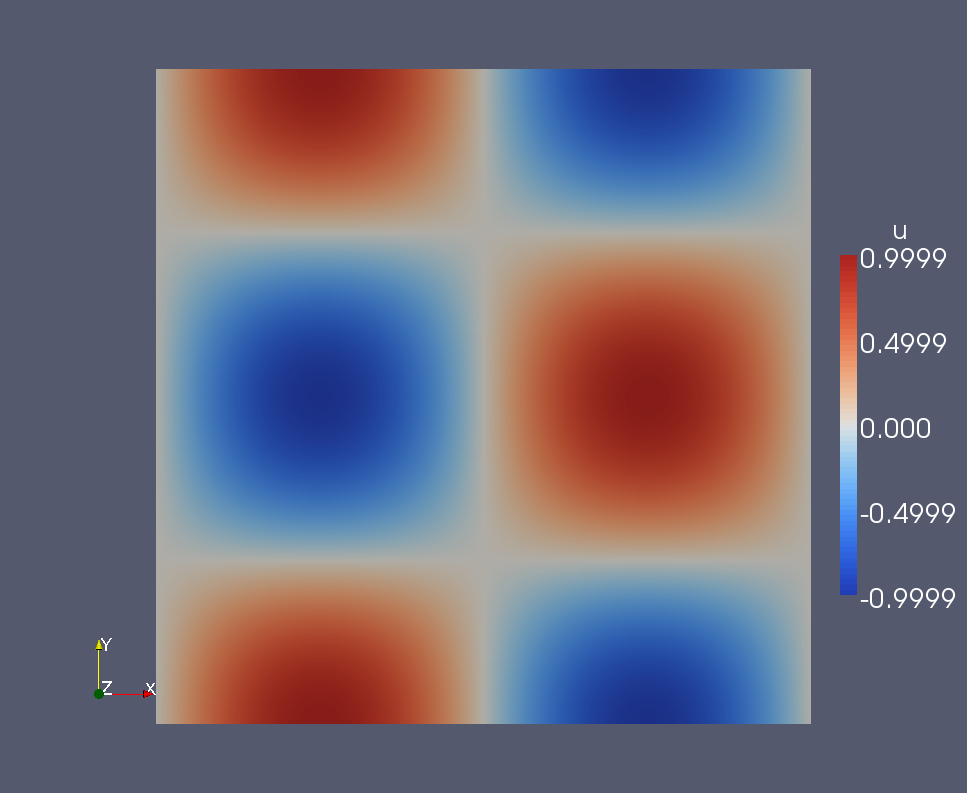
\includegraphics[width=.43\linewidth]{laplacian.png}}
  \subfigure[Elevation]{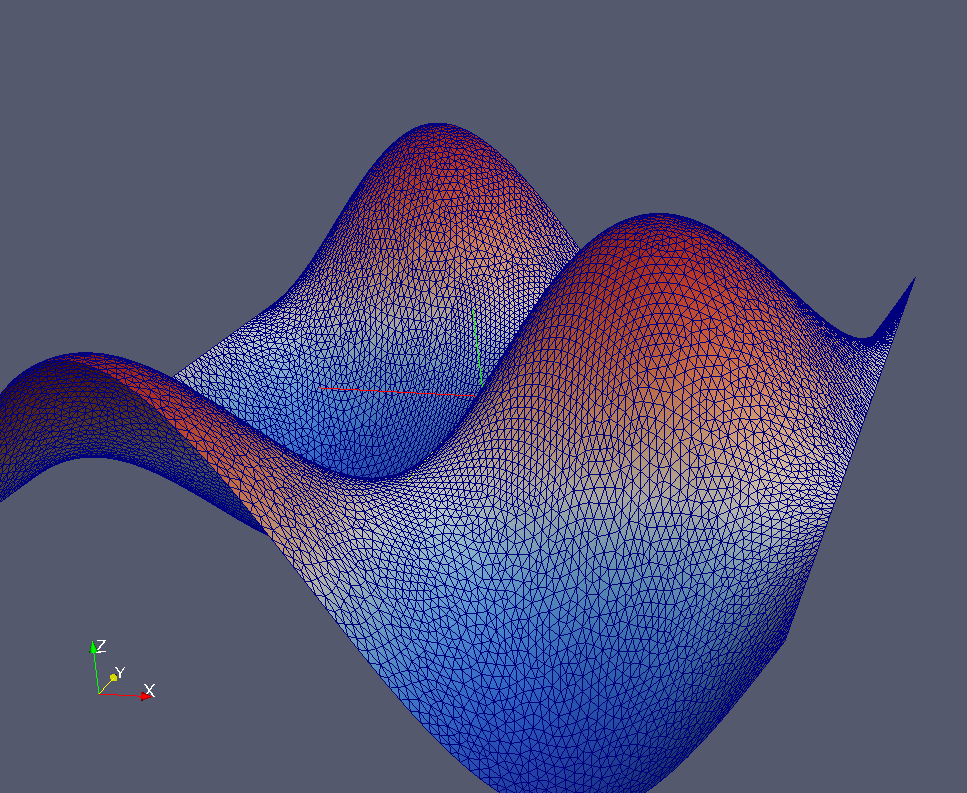
\includegraphics[width=.43\linewidth]{laplacian_warp.png}}
  \caption{Solution of problem~\ref{prob:3}}
  \label{fig:2}
\end{figure}

%%%%%%%%%%%%%%%%%%%%%%%%%%%%%%%%%%%%%%%%%%%%%%%%%%%%%%%%%%%%%%%%%%%%%%%%%%%%%%%%%%%%%%%%
Let's try a parallel computation using 3 processors. The following figures display the results using Paraview.
\begin{remark}
 You can modify the domain size in order to obtain a clearer figure by adding diffrent values to \lstinline!_xmin!    \lstinline!_ymin!   \lstinline!_xmax! and  \lstinline!_ymax!  in the definition of the mesh in \lstinline!laplacian.cpp!
 \end{remark}

 \begin{figure}[!h]%[htbp]
  \centering
  \subfigure[domain 1]{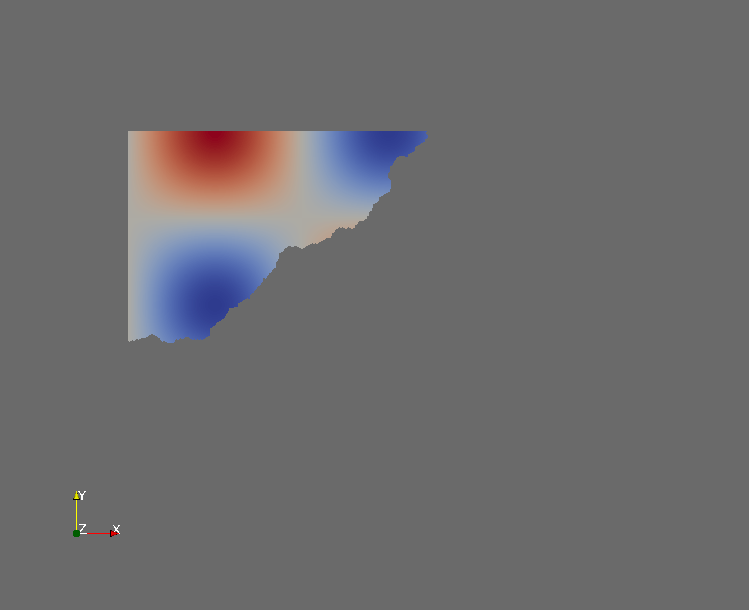
\includegraphics[width=.43\linewidth]{pngs/laplacian/laplacian_1.png}}
  \subfigure[domain 2]{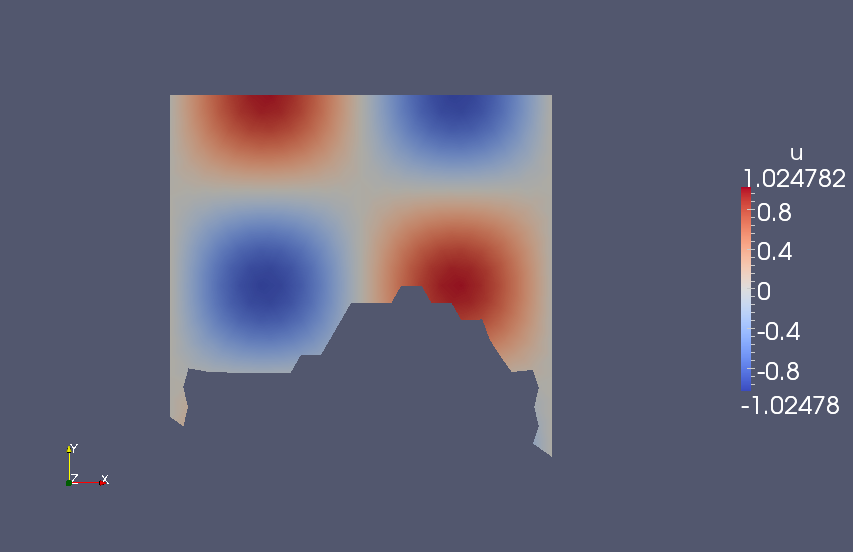
\includegraphics[width=.43\linewidth]{pngs/laplacian/laplacian_2.png}}\\
  \subfigure[domain 3]{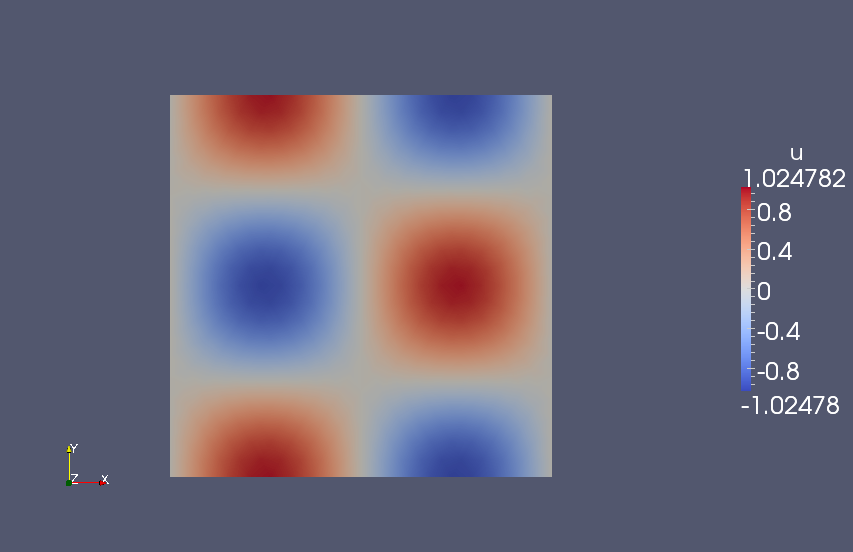
\includegraphics[width=.43\linewidth]{pngs/laplacian/laplacian_3.png}}
  \subfigure[partition colored with pid]{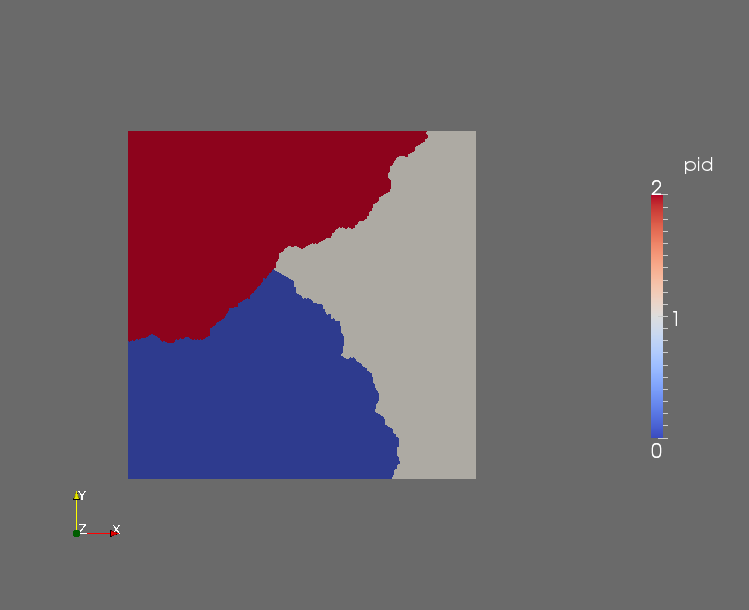
\includegraphics[width=.43\linewidth]{pngs/laplacian/laplacian_Pid.png}}
  \caption{Solution of the laplacian problem}
  \label{fig:2}
\end{figure}
%%%%%%%%%%%%%%%%%%%%%%%%%%%%%%%%%%%%%%%%%%%%%%%%%%%%%%%%%%%%%%%%%%%%%%%%%%%%%%%%%%%%%%%%


\newpage

\subsection{Mixed formulation: the Stokes case}
\label{sec:mixed-form-stok}
\index{Stokes}
\subsubsection{Mathematical formulation}
\label{sec:math-form}

\index{Stokes!formulation!mathematical}
\marginpar{\lstinline!stokes.cpp!}  We are now interested in solving
the Stokes equations, we would like to solve for the following problem
in 2D
\begin{problem}
\label{prob:4}
 find $(\mathbf{u},p)$ such that
\begin{equation}
  \label{eq:22}
  - \mu \Delta \mathbf{u} +\nabla p = \mathbf{f}\quad \text{and}\quad \nabla \cdot \mathbf{u} = 0,\quad \text{in}\ \Omega = [-1;1]^2
\end{equation}
with
\begin{equation}
  \label{eq:24}
  \mathbf{f} = \mathbf{0}
\end{equation}
where $\mu$ being the viscosity. The following boundary conditions apply
\begin{equation}
  \label{eq:23}
  \mathbf{u}=\mathbf{1}_{|y=1}, \quad \mathbf{u}=\mathbf{0}_{|\partial \Omega \backslash \{(x,y) \in \Omega | y=1\}}
\end{equation}
\end{problem}

In problem (\ref{prob:2}), $p$ is known up to a constant $c$,
\emph{i.e.} if $p$ is a solution then $p+c$ is also solution. To
ensure uniqueness we impose the constraint that $p$ should have
zero-mean, \emph{i.e.}
\begin{equation}
  \label{eq:26}
  \int_\Omega p = 0
\end{equation}

The problem~\ref{prob:4} now reads
\begin{problem}
  \label{prob:5}
 find $(\mathbf{u},p,\lambda)$ such that
\begin{equation}
  \label{eq:34}
  - \mu \Delta \mathbf{u} +\nabla p = \mathbf{f}\quad, \quad \nabla \cdot \mathbf{u} + \lambda = 0, \quad \text{and}\quad \int_\Omega p = 0,\quad \text{in}\ \Omega = [-1;1]^2
\end{equation}
with
\begin{equation}
  \label{eq:35}
  \mathbf{f} = \mathbf{0}
\end{equation}
where $\mu$ being the viscosity. The following boundary conditions apply
\begin{equation}
  \label{eq:36}
  \mathbf{u}=\mathbf{1}_{|y=1}, \quad \mathbf{u}=\mathbf{0}_{|\partial \Omega \backslash \{(x,y) \in \Omega | y=1\}}
\end{equation}
\end{problem}

The functional framework is as follows, we look for $\mathbf{u}$ in
$H^1_0(\Omega)$ and $p$ in $L^2_0(\Omega)$. We shall not seek $p$ in
$L^2_0(\Omega)$ but rather in $L^2(\Omega)$ and use Lagrange
multipliers which live are the constants whose space we denote
$\mathbb{P}_0(\Omega)$, to enforce~(\ref{eq:26}).

Denote $\mathcal{X} = H^1_0(\Omega)\times
L^2(\Omega)\times\mathbb{P}_0(\Omega)$, the variational formulation
reads we look for $(\mathbf{u}, p, \lambda) \in \mathcal{X}$ for all
$(\mathbf{v},q,\nu) \in \mathcal{X}$
\begin{equation}
  \label{eq:25}
  \int_\Omega \mu \nabla \mathbf{u} : \nabla \mathbf{v} + \nabla \cdot \mathbf{v} p + \nabla \cdot \mathbf{u}\ q + q \lambda + p \nu  \ = \ \int_\Omega \mathbf{f} \cdot \mathbf{v}
\end{equation}

We build a triangulation $\Omega_h$ of $\Omega$, we choose compatible
(piecewise polynomial) discretisation spaces $X_h$ and $M_h$,
\emph{e.g.} the Taylor Hood element ($\mathbb{P}_N/\mathbb{P}_{N-1}$)
and we denote $\mathcal{X}_h=X_h\times M_h \times
\mathbb{P}_0(\Omega)$.  The discrete problem now reads, we look for
$(\mathbf{u}_h,p_h,\lambda_h) \in \mathcal{X}_h$ such that for all
$(\mathbf{v}_h,q_h,\nu_h) \in \mathcal{X}_h$
\begin{equation}
  \label{eq:27}
  \int_{\Omega_h} \mu \nabla \mathbf{u}_h \cdot \nabla \mathbf{v}_h + \nabla \cdot \mathbf{v}_h \ p_h + \nabla \cdot \mathbf{u}_h\ q_h + p_h \nu_h + q_h \lambda_h   = \ \int_{\Omega_h} \mathbf{f} \cdot \mathbf{v}_h
\end{equation}

The formulation~(\ref{eq:27}) leads to a linear system of the form
\begin{equation}
  \label{eq:28}
  \underbrace{\begin{pmatrix}
    A & B & 0\\
    B^T & 0 & C\\
    0 & C^T & 0
  \end{pmatrix}}_{\mathcal{A}}
\underbrace{
  \begin{pmatrix}
    \mathbf{u}_h\\
    p_h\\
    \lambda_h
  \end{pmatrix}}_{\mathcal{U}} =
\underbrace{\begin{pmatrix}
    F\\
    0\\
    0
  \end{pmatrix}}_{\mathcal{F}}
\end{equation}

where $A$ corresponds to the $(\mathbf{u},\mathbf{v})$ block, $B$ to
the $(\mathbf{u},q)$ block and $C$ to the $(p,\nu)$
block. $\mathcal{A}$ is a symetric positive definite matrix and thus
the system $\mathcal{A} \mathcal{U} = \mathcal{F}$ enjoys a unique
solution.

\subsubsection{Feel formulation}
\label{sec:feel-formulation}

\index{Stokes!formulation!feel}
Regarding the implementation of the Stokes problem~\ref{prob:4}, we
can start from the laplacian case, from
section~\ref{sec:defin-bilin-forms}. The implementation we choose to
display here defines and builds $\mathcal{X}_h$, $\mathcal{A}$,
$\mathcal{U}$ and $\mathcal{F}$.

We start by defining and building $\mathcal{X}_h$: first we define the
basis functions that will span each subspaces $X_h$, $M_h$ and
$\mathbb{P}_0(\Omega)$.

\lstinputlisting[linerange=marker1-endmarker1]{tutorial/stokes.cpp}

note that on the \lstinline!typedef! we build a (MPL) vector of them. Now we are
ready to define the functionspace $\mathcal{X}_h$, much like in the
Laplacian case:

\lstinputlisting[linerange=marker2-endmarker2]{tutorial/stokes.cpp}

Next we define a few types which are associated with $\mathcal{U}$,
$u$, $p$ and $\lambda$ respectively.

\lstinputlisting[linerange=marker3-endmarker3]{tutorial/stokes.cpp}

Using these types we can instantiate elements of $\mathcal{X}_h$,
$X_h$, $M_h$ and $\mathbb{P}_0(\Omega_h)$ respectively:

\lstinputlisting[linerange=marker4-endmarker4]{tutorial/stokes.cpp}

They will serve in the definition of the variational formulation. We
can now start assemble the various terms of the variational
formulation~(\ref{eq:27}). First we define some viscous stress tensor,
%$\tau(\mathbf{u}) = \frac{1}{2}(\nabla \mathbf{u} + \nabla \mathbf{u}^T)$,
$\tau(\mathbf{u}) = \nabla \mathbf{u}$,
associated with the trial and test functions
respectively

\lstinputlisting[linerange=marker5-endmarker5]{tutorial/stokes.cpp}

Then we define the total stress tensor times the normal,
$\bar{\sigma}(\mathbf{u},p) \mathbf{n} = -p \mathbf{n} + 2 \mu \tau(\mathbf{u})
\mathbf{n}$ where $\mathbf{n}$ is the normal and $\bar{\sigma}(\mathbf{u},p) =
-p \mathbb{I} + 2 \mu \tau(\mathbf{u})$:

\lstinputlisting[linerange=marker6-endmarker6]{tutorial/stokes.cpp}


We then form the matrix $\mathcal{A}$ starting with block $A$,  block $B$
block $C$ and finally the boundary conditions.


\lstinputlisting[linerange=marker7-endmarker7]{tutorial/stokes.cpp}

The figure~\ref{fig:2} displays $p$ and $\mathbf{u}$ which are available in
\begin{unixcom}
  ls ~/feel/doc/tutorial/stokes/Simplex_2_1_2/P2/h_0.05
\end{unixcom}

\begin{figure}[htbp]
  \centering
  \subfigure[Colored with $p$, $h=0.05$]{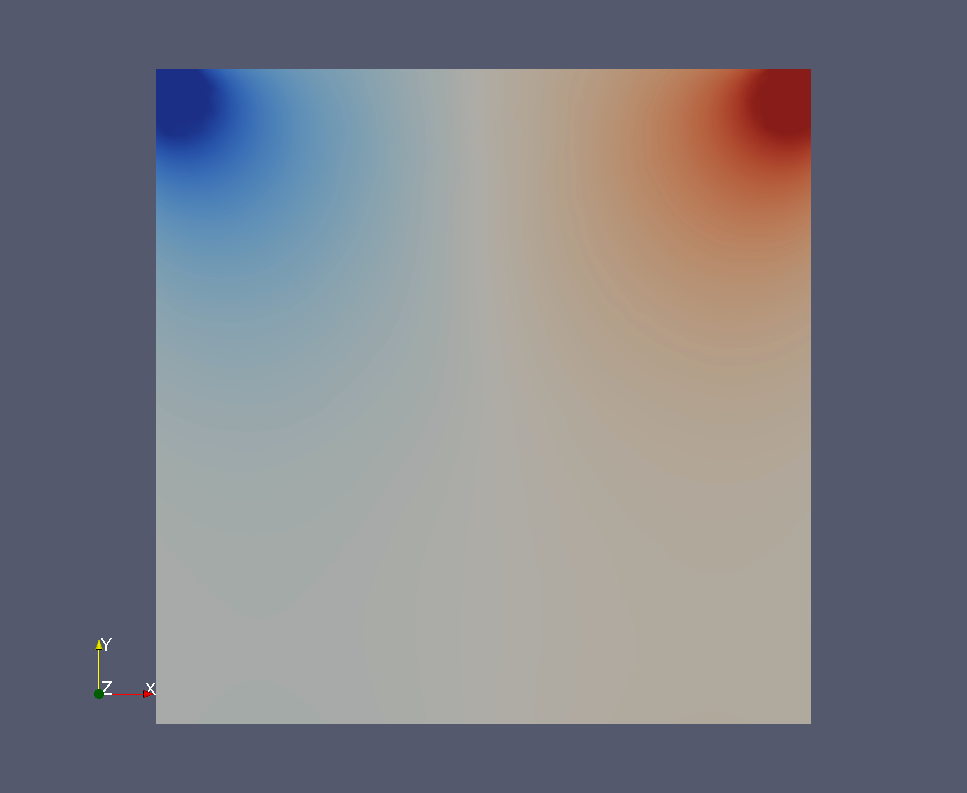
\includegraphics[width=.43\linewidth]{stokes-p.png}}
  \subfigure[Colored with $\|\mathbf{u}\|$ and the arrows associated to $\mathbf{u}$ colored with $p$]{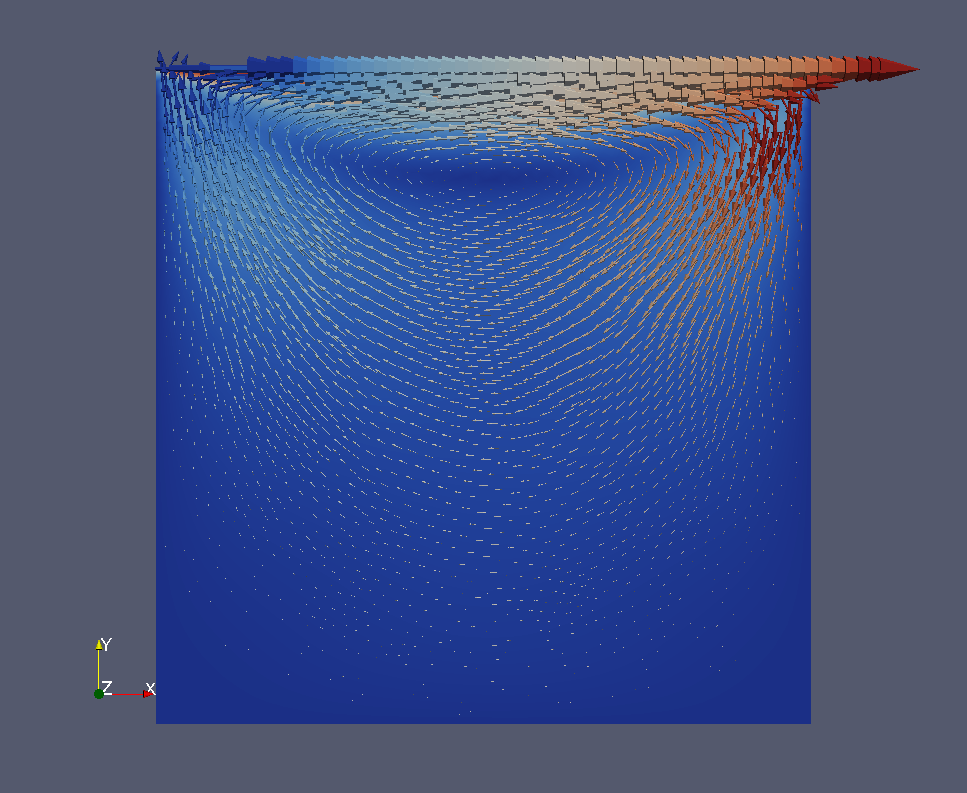
\includegraphics[width=.43\linewidth]{stokes-u.png}}
  \caption{Solution of problem~\ref{prob:4}}
  \label{fig:2}
\end{figure}

%%% Local Variables:
%%% coding: utf-8
%%% mode: latex
%%% TeX-PDF-mode: t
%%% TeX-parse-self: t
%%% x-symbol-8bits: nil
%%% TeX-auto-regexp-list: TeX-auto-full-regexp-list
%%% TeX-master: "../feel-manual"
%%% ispell-local-dictionary: "american"
%%% End:

